\dev{Emile Martinez}{Balabonski, Barra}

La mémoire d'un programme meurt avec lui. Néanmoins, on souhaite garder des données plus perennement.

La mémoire d'un ordinateur est alors une série de milliards de bits, parmi lesquels coexistent tout et n'importe quoi. On veut les organiser de façon à rendre leur accès le plus simple et rapide possible.

\section{Fichiers}

\subsection{Organisation et manipulation}

\begin{definition}
	Un fichier est un ensemble de données. C'est l'unité de stockage manipulé par l'utilisateur.
\end{definition}

\begin{definition}
	Pour organiser des données de manière persistante sur un disque on utilise une arborescence de fichier. La norme POSIX, suivie par la plupart des OS (linux, Mac, android) définit cette organisation et sa manipulation.
\end{definition}

\begin{example}
	Arborescence de fichier linux (obtenue par la commande \texttt{tree})\\
	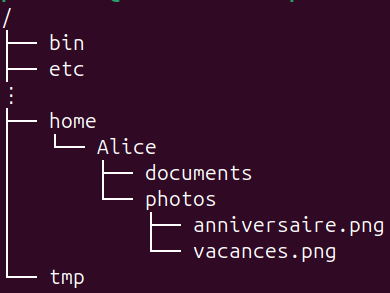
\includegraphics[width=0.4\linewidth]{lecon/21-fichier/arborescence.png}
\end{example}

\begin{definition}
	Le chemin d'accès vers un fichier est soit exprimé de manière absolu (depuis la racine) soit depuis le répertoire courant
\end{definition}

\begin{impl}
	On peut accèder et manipuler l'arborescence de fichier depuis un invite de commande (shell ou terminal) avec les commandes suivantes : \begin{itemize}[label=$\bullet$]
	\item pwd : affiche le repertoire courant
	\item cd chemin : change le repertoire courant pour la cible du chemin
	\item mkdir/touch : créer un dossier/un fichier
	\item cp/mv/rm : copie/ déplace et renomme / supprime
	\item ls  : liste le contenu d'un repertoire
	\end{itemize}
\end{impl}

\begin{exercise}
	Prise en main des commandes du shell avec appuie sur l'utilisation du man.
\end{exercise}

\begin{impl}
	La commande ls -l permet de faire apparaitre des informations supplémentaires sur les fichiers : propriétaire, groupe prioritaire, taille, dernière modification et autorisations :
	\normalfont
	$$ \underset{\circled{1}}{\underbrace{\texttt{\enspace\enspace-}}} \underset{\circled{2}}{\underbrace{\texttt{rwx}}}\underset{\circled{3}}{\underbrace{\texttt{r--}}}\underset{\circled{4}}{\underbrace{\texttt{r--}}}$$
	
	$\circled{1}$ : type de fichier : \begin{itemize}
		\item[] \qquad \texttt{d} : répertoire
		\item[] \qquad \texttt{l} : lien symbolique
		\item[] \qquad \texttt{-} : autre
	\end{itemize}
	
	$\circled{2}\circled{3}\circled{4}$ : \begin{itemize}
		\item[] \qquad \texttt{r} : read
		\item[] \qquad \texttt{w} : write
		\item[] \qquad \texttt{x} : execute
	\end{itemize}
	
	$\circled{2}$ : permissions propriétaire
	
	$\circled{3}$ : permissions groupe
	
	$\circled{4}$ : permissions tous
	
	
\end{impl}

\begin{rem}
	Pour Linux, "tout est un fichier" : les codes sources, les exécutables, mais aussi les périphériques qui peuvent être lus (souris, clavier) ou écrits (écran) comme des fichiers
\end{rem}

\begin{proposition}
	Plusieurs systèmes de fichiers (volume dans la mémoire) peuvent cohabiter sur un même ordinateur, avec chacun leur racine
\end{proposition}

\begin{example}
	Les C::, D::, E::, etc. sous Windows sont autant de système de fichiers
\end{example}

\begin{rem}
	Sous Linux, tous les espaces de stockages montés partagent la même arborescence
\end{rem}

\subsection{Stockage}

Il existe plusieurs manières de faire un système de fichier (FAT32, ext4, \dots) définissant des primitives de gestion des fichiers ainsi que des structures de données pour la gestion des espaces libres.

\begin{definition}
	On découpe alors les fichiers en blocs de quelques ko. Le système de fichier ne manipulera alors que des blocs.
\end{definition}

\begin{definition}
	Un fichier étant souvent trop grand pour un unique bloc, il est séparé en plusieurs blocs : \begin{itemize}
	
	\item allocation contigüe : les blocs sont contigües sur le disque \\
	$\to$ accès séquentiel rapide mais fragmentation et difficulté à créer ou etendre des fichiers.
	
	\item allocation chaînée : les blocs peuvent être n'importe où, chaque bloc contenant l'adresse du suivant\\
	$\to$ bonne utilisation de la mémoire, création extension facile mais accès séquentiel lent
	
	On dispose alors parfois d'une table d'allocation de fichiers
	
	\item l’allocation indexée : les adresses des blocs constituant un même fichier sont rangées dans une table, appelée index, elle-même con
	
	tenue dans un ou plusieurs blocs.
	
	$\to$ bonne accès séquentiel et extension facile, mais taille de fichier maximales et utilisation de mémoire annexe (visible surtout sur les petits fichiers)
	\end{itemize}
\end{definition}


\begin{definition}
	Chaque fichier se voit associé un numéro inode à un emplacement de stockage. L'inode permet de retrouver dans une table du périphérique de stockage des infos données par \texttt{ls -l}.
\end{definition}

\begin{definition}
	Pour économiser de la place, des liens peuventêtre crées entre des fichiers avec :
	
	\qquad \texttt{ln} : lien physique, l'inode est partagé mais la suppression d'un des fichiers n'impacte pas l'autre
	
	\qquad \texttt{ln -s} : lien symbolique, un nouvel inode est utilisé et le fichier ne contient que le chemin vers sa source.

\end{definition}

\section{Format}

\subsection{Fichier texte}

\begin{definition}
	Un fichier texte représente uniquement une suite de caractères (type char en C ou en OCaml) codé en ASCII.
\end{definition}

\begin{rem}
	C'est le format de fichier de base.
\end{rem}

\begin{rem}
	Il arrive que l'on veuille représenter plus que les 128 caractères qu'autorise l'ASCII (ou 256 pour l'ASCII étendue). On peut alors utiliser des codages sur plus de bits (16 pour l'unicode par exemple).
\end{rem}

\begin{definition}
	Étant le format de fichier le plus basique, il est le plus simple à manipuler. On pourra alors accéder à ces fichiers en langage de programmation :\\
	\begin{tabular}{l|l|l}
		\multicolumn{1}{c}{Fonction} & \multicolumn{1}{|c|}{En C} & \multicolumn{1}{c}{En OCaml}\\
		ouvrir un fichier &  \texttt{fopen(chemin, mode)} & \texttt{open\_in} \\
		fermer un fichier & \texttt{fclose(fichier)} & \texttt{close\_in} \\
		écrire dans un fichier & \texttt{fprintf} & \texttt{input\_line} \\
		lire dans un fichier & \texttt{scanf} & \texttt{output\_line}
	\end{tabular}
\end{definition}

\begin{rem}
	Lorsqu'on utilise \texttt{printf} en C, on écrit dans un fichier particulier : la sortie standard (stdout) qui correspond à l'invite de commande. \texttt{printf} est donc équivalent à \texttt{fprintf(stdout, $\dots$)}. De même, \texttt{scanf} lit dans l'entrée standard (stdin). 
\end{rem}

\begin{definition}
	Pour rediriger la sortie standard, on peut utiliser des commandes : \begin{itemize}
		\item \texttt{commande > filename} : la sortie standard de la commande est écrite ddans le fichier, qui est écrasé.
		\item \texttt{commande >> filemane} : même chose mais sans écraser le fichier. 
		\item \texttt{commande < fichier} : le fichier devient l'entrée standard de la commande
		\item \texttt{commande1 | commande2} : la sortie standard de la première commande est reliée à l'entrée standard de la deuxieme.
	\end{itemize}
\end{definition}

\begin{rem}
	L'écriture étant lente, un tampo est utilisé. On peut forcer l'écriture des tampons avec \texttt{flush} en OCaml et \texttt{fflush} en C.
\end{rem}

\subsection{Formats de fichiers}

Pour représenter plus que des chaînes caractères, on a besoin de définir des formats de fichiers qui indiquent comment interpréter les bits de données. 

\begin{definition}
	Un format de fichier est une convention de représentation de données
\end{definition}

\begin{rem}
	Pour gagner de l'espace, ces formats utilisent souvent des méthodes de compression, avec ou sans perte.
\end{rem}

\begin{example}
	Quelques formats particuliers :
	\begin{itemize}
		\item Le format png stocke et compresse les images sans perte
		\item Le format jpeg stocke des images compressées avec perte
		\item Le formats mp3 stocke des sons compressés avec perte
		\item Le format mp4 combine audio et vidéo
		\item Le format zip compresse sans perte des fichiers quelconques
	\end{itemize}
\end{example}

\begin{rem}
	Le format zip utilise l'algorithme de compression LZW, mais aussi le codage de Huffman.
\end{rem}

\paragraph{Développement :} Présentation de l'algorithme LZW.

\begin{rem}
	Il y a toujours un compromis à faire entre différents objectifs (ex : compression et facilité d'utilisation). Ainsi la plupart des formats se spécialisent dans une utilisation :
	\begin{itemize}
		\item quand on ouvre une image en python, on la transforme en tableau de triplets, quand on la sauvegarde on la recompresse, dans un format moins manipulable
		\item Quand on édite une vidéo, on doit l'exporter à la fin pour passer d'un format manipulable à un format pour la lecture
		\item Quand on compresse des fichiers en .zip, on ne peut plus les modifier ou les lire 
	\end{itemize}raison pour lesquelles on exporte quand on monte une vidéo, pour baser d'un format éditable à un format compressé adapté à la lecture).
\end{rem}

\begin{example}
	Le format CSV (pour comma separated values) est un format de texte brut permettant de stocker des données sous forme de table, permettant ainsi facilement la suppresion, l'ajout, etc.\\
	
	Pour des commandes \{ produit : tomate, prix : 3 quantité : 50, client : Le navet naviguant, adresse : 13 rue du Swag à Tarbes \},  \{ produit : patate, prix : 1, quantité : 30, client : Le navet naviguant, adresse : 13 rue du Swag à Tarbes \},  \dots
	
	Pourrait-on mieux faire ?
\end{example}

\section{Bases de données}

Souvent, les données d'une table ont des redondances, et des liens entre elles (cf exemple au dessus). Pour manipuler des gros volumes de données on ne se contente alors plus alors de fichiers en texte brut.

\begin{definition}
	Le modèle relationnel est une manière de représenter les données en exploitant les relations entre elles.
\end{definition}

\begin{example}
	Un grossistes gérant des commandes.
	\texttt{Produit(\underline{num\_produit}, nom, prix, poids)}\\
	\texttt{Clients(\underline{num\_client}, nom, adresse, ville)}\\
	\texttt{Commande(\underline{\#num\_produit, \#num\_client}, quantite)}\\
	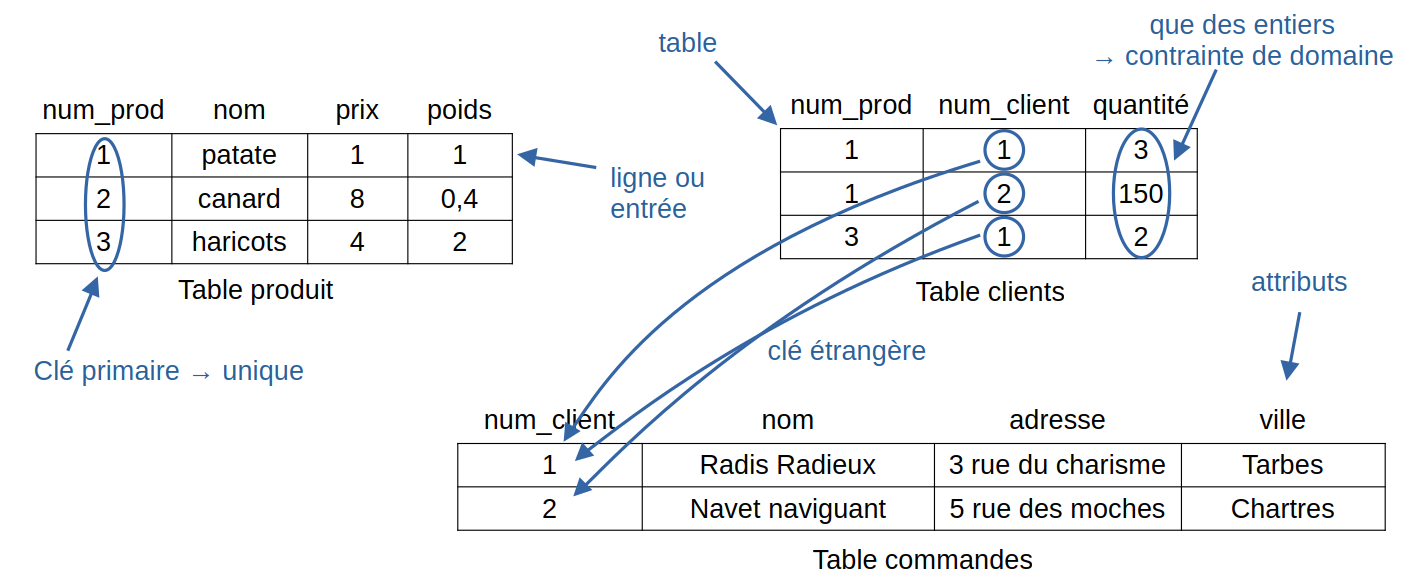
\includegraphics[width=\linewidth]{lecon/21-fichier/schema_bd.png}
\end{example}

\begin{definition}
	Un SGBD (système de gestion de bases de données) est utilisé pour manipuler des données relationnelles, garantissant les propriétés ACID (atomicité, cohérence, isolation et durabilité). On intéragit avec lui à travers le langage SQL.
\end{definition}

\begin{example}
	Le SQL permet de sélectionner certaines données, de les trier, de les filtrer selons certaines conditions, etc \dots
\end{example}

\begin{com}
	Si on a la place ici, on peut insérer des mots clés.
\end{com}

\begin{theorem}[Codd]
	SQL est suffisamment expressif pour quasiment tout ce que l'on souhaite faire
\end{theorem}

\begin{exercise}
	Trouver différentes manières de calculer le max et la division.
\end{exercise}

\paragraph{Développement :} Correction de l'exercice précédent.

\begin{com}
	Ici on pourrait également défendre le fait de faire plutôt l'autre développement de requêtes SQL, introduisant les requêtes, les mots clés de bases, etc. Il s'insère parfaitement dans la leçon, (mieux que ce développement là où il faut justifier que on a introduit aucune syntaxe dans le cours, mais que en vrai ils la connaîtraient), mais c'est un développement moins poussé. Donc on montre moins la puissance de calcul.
\end{com}

